
\documentclass[12pt,a4paper]{book}

\usepackage{geometry}
\usepackage{amsmath,amssymb}

\usepackage{xcolor}

\usepackage{tikz,pgfplots}
\pgfplotsset{compat=1.12}
\usepgfplotslibrary{fillbetween}
\usetikzlibrary{patterns}
\usetikzlibrary{positioning}
\usetikzlibrary{arrows,automata}
\usepackage{cancel}
\def\checkmark{\tikz\fill[scale=0.4](0,.35) -- (.25,0) -- (1,.7) -- (.25,.15) -- cycle;} 

\begin{document}
$5.$ Find the equivalent partition of the following machine.
\begin{center}
\begin{table}[h]
\centering
\scalebox{1.5}{
\begin{tabular}{lllr}
\hline
&\multicolumn{3}{c}{Next State,z} \\
\cline{2-4}
\centering
Present State   &$X=0$  & $X=1$ \\
\hline
A &C, 1 &D, 0\\
B &D, 1 &E, 0\\
C &B, 1 &E, 1\\
D &B, 1 &A, 0\\
E &D, 1 &B, 1\\
\hline
\end{tabular}
}
\end{table}
\end{center}
\textbf{Solution:}  The partitions are\\
$P_0$ = (ABCDEF)\\
$P_1$ = (AD)(BCE) (Depending on o/p for i/p 1)\\
$P_2$ = (AD)(BE)(C) (For i/p 0, the next state of C goes to another set)\\
$P_3$ = (A)(D)(BE)(C) (For i/p 0, the next state of A and D goes to a different set)\\
$P_4$ = (A)(D)(BE)(C)\\
As $P_3$ and $P_4$ are the same, $P_3$ is the equivalent partition.\\
\textbf{ Minimization:} We know that the equivalent partition is unique. So,\\ $P_4$ = (A)(D)(BE)(C) is the
unique combination. Here, every single set represents one state of the minimized machine.\\
Let us rename these partitions for simplifi cation.\\
Rename (A) as $S_1$, (BE) as $S_2$, (C) as $S_3$, and (D) as $S_4$.\\
The minimized machine becomes
\begin{center}
\begin{table}[h]
\centering
\scalebox{1.5}{
\begin{tabular}{lllr}
\hline
&\multicolumn{3}{c}{Next State,z} \\
\cline{2-4}
\centering
Present State   &$X=0$  & $X=1$ \\
\hline
$S_1$(A) &$S_3$, 1 &$S_4$, 1\\
$S_2$(BE) &$S_4$, 1 &$S_2$, 0\\
$S_3$(C) &$S_2$, 1 &$S_2$, 1\\
$S_4$(D) &$S_2$, 1 &$S_1$, 0\\
\hline
\end{tabular}
}
\end{table}
\end{center}
$6.$ Simplify the following incompletely specifi ed machine.
\begin{center}
\begin{table}[h]
\centering
\scalebox{1.5}{
\begin{tabular}{llllr}
\hline
&\multicolumn{3}{c}{Next State,z} \\
\cline{2-4}
\centering
Present State   &$I_1$  & $I_2$ &$I_3$ \\
\hline
A &D, 1 &E,1 &$-$ \\
B &B, 0 &E,$-$ &C,$ -$\\
C &C, $-$ &C,0 &B, $-$\\
D &B, 0 &D,$-$ &E,$-$\\
E & $-$ &B,0 &A, $-$\\
\hline
\end{tabular}
}
\end{table}
\end{center}
\textbf{Solution:}  Put a temporary state T in the next state place, where the next states are not specifi ed.
If the output is not mentioned, there is no need to put any output.
\newpage
As a temporary state T is considered, T is put in the present state column with the next state T for all inputs with no output.\\
The simplifi ed machine becomes\\
\begin{center}
\begin{table}[h]
\centering
\scalebox{1.5}{
\begin{tabular}{lllr}
\hline
&\multicolumn{3}{c}{Next State,z} \\
\cline{2-4}
\centering
Present State   &$I_1$  & $I_2$ &$I_3$ \\
\hline
A &D, 1 &E,1 &T,$-$ \\
B &B, 0 &E,$-$ &C,$ -$\\
C &C, $-$ &C,0 &B, $-$\\
D &B, 0 &D,$-$ &E,$-$\\
E &T, $-$ &B,0 &A, $-$\\
T &T, 0 &T,0 &T,0\\
\hline
\end{tabular}
}
\end{table}
\end{center}
$7.$ Minimize the following incompletely specifi ed machine.\\
\begin{center}
\begin{table}[h]
\centering
\scalebox{1.5}{
\begin{tabular}{lllr}
\hline
&\multicolumn{3}{c}{Next State,z} \\
\cline{2-4}
\centering
Present State   &$I_1$ & $I_2$ &$I_3$ \\
\hline
A &A, 1 &D, $-$ &C,$-$\\
B &A, $-$ &D, $-$ &E,$-$\\
C &E, 0 &A, 1 &$-$,$-$\\
D &E, $-$ &A, 1 &$-$,$-$\\
E &E, 0 &$-$, $-$ &C,$-$\\
\hline
\end{tabular}
}
\end{table}
\end{center}
\textbf{Solution:}  In an incompletely specifi ed machine, all the next states or all the outputs or both are not
mentioned. We can minimize an incompletely specifi ed machine by using the merger graph and
compatible graph method. From the merger graph, we have to fi nd the compatible pair and from that
compatible pair and implied pair we have to construct compatible graph. From the compatible graph,
we have to fi nd the closed partition. And, the closed partitions are the minimized states of the machine.\\
\textbf{Merger Graph:}  The machine consists of fi ve states. So, the merger graph consists of fi ve nodes,
named A, B, C, D, and E.\\ The outputs of A and B do not differ, and so there is an arc between A and
B. For input I3, the next state confl icts. so the arc
is an interrupted arc and in the interrupted portion
the confl icting next state pair (CE) is placed.\\
For states A and C, the output confl icts, and so
there is no arc between A and C.\\
For the states C and D, the outputs as well as
next states do not confl ict. So, an uninterrupted
arc is placed between C and D.\\
By this process, the merger graph is constructed.\\
The merger graph is as follows
As there is no arc between A and E, the
arc between (AD), (BE), (BD), and (BC) are
also crossed.
\begin{center}
  \begin{tikzpicture}[node distance=3.5cm]
  \node[state] (e)   {$E$}; 
   \node[state] (a) [above right=of e] {$A$}; 
   \node[state] (b) [right=of e] {$B$}; 
   \node[state] (d) [below=of e] {$D$}; 
   \node[state] (c) [right=of d] {$C$}; 
    \draw (e) -- ++(b) node [midway,fill=white] {\xcancel{(AE)(CE)}};
   \draw (e) -- ++(c) node [midway,fill=white] {\xcancel{(AE)(AD)}};
   \draw (e) -- ++(d) node  {};
   \draw (a) -- ++(d) node [midway,fill=white] {\xcancel{(AE)}};
   \draw (b) -- ++(c) node [midway,fill=white] {\xcancel{(AE)(AD)}};
   \draw (a) -- ++(b) node [midway,fill=white] {(CE)};
   \draw (d) -- ++(c) node  {};
  \end{tikzpicture}
\end{center}

\textbf{Compatible Graph:}  (CE) is the implied pair for (AB). A
directed arc is drawn from (AB) to (CE). The compatible
graph consists of four vertices (AB), (CD), (DE), and (CE).\\
A subgraph of a compatibility graph is said to be closed
cover for the machine, if for every vertex in the subgraph, all
outgoing edges and their terminal vertices also belong to the
subgraph, and every state of the machine is covered by at least
one vertex of the subgraph.\\
\begin{center}
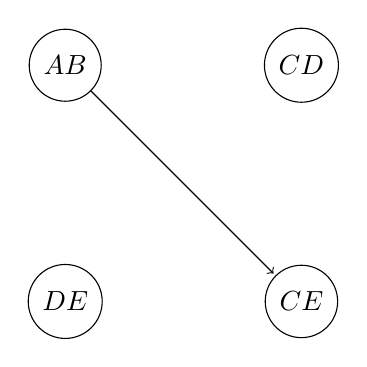
\begin{tikzpicture}[shorten >=1pt,node distance=3cm,on grid,auto]
  \node[state] (q0)   {$AB$}; 
   \node[state] (q1) [right=of q0] {$CD$}; 
   \node[state] (q2) [below=of q0] {$DE$}; 
   \node[state](q3) [below=of q1] {$CE$};
   \path[->] (q0) edge node {} (q3);
 \end{tikzpicture}
 \end{center}
 For the constructed compatible graph, (AB), (CD), and
(CE) form a closed covering.\\ The states of the minimized machine are (AB) and (CDE).\\ Rename
(AB) as $S_1$ and (CDE) as $S_2$.\\
The minimized machine is
 \begin{center}
\begin{table}[h]
\centering
\scalebox{2}{
\begin{tabular}{lllr}
\hline
&\multicolumn{3}{c}{Next State,z} \\
\cline{2-4}
\centering
Present State   &$I_1$ & $I_2$ &$I_3$ \\
\hline
$S_1$ &$S_1$, 1 &$S_2$, $-$ &$S_2$, $-$\\
$S_2$ &$S_2$, 0 &$S_1$, 1 &$S_2$, $-$\\
\hline
\end{tabular}
}
\end{table}
\end{center} \newpage
$8.$ Construct a compatible graph for the following incompletely specifi ed machine.
\begin{center}
\begin{table}[h]
\centering
\scalebox{1.5}{
\begin{tabular}{llllr}
\hline
&\multicolumn{4}{c}{Next State,z} \\
\cline{2-5}
\centering
Present State   &$I_1$ & $I_2$ &$I_3$ &$I_4$ \\
\hline
A &A, $O_1$ &E, $O_2$ &$-$, $-$ &A, $O_2$\\
B &$-$, $-$ &C, $O_3$ &B, $O_1$ &D, $O_4$\\
C &A, $O_1$ &C, $O_3$ &$-$, $-$ &$-$, $-$\\
D &A, $O_1$ &$-$, $-$ &$-$, $-$ &D, $O_4$\\
E &$-$, $-$ &E, $O_2$ &F, $O_1$ &$-$, $-$\\
F &$-$, $-$ &G, $O_3$ &F, $O_1$ &G, $O_4$\\
G &A, $O_1$ &$-$, $-$ &$-$, $-$ &G, $O_4$\\
\hline
\end{tabular}
}
\end{table}
\end{center}
\textbf{Solution:}  To construct a compatible graph, we have to fi rst fi nd compatible pairs. To fi nd the
compatible pairs, we need to construct a merger graph. But this machine has seven states, and so
it is diffi cult to construct a merger graph for this machine. So, we have to construct a merger table
to fi nd compatible pairs.
\begin{table} 
\begin{center}
\scalebox{1.5}{
 \begin{tabular}{lllllllr} 
 \cline{2-2}
 B   &\multicolumn{1}{|c}{$\times$}&\multicolumn{6}{|c}{} \\ 
\cline{2-3}
 C &\multicolumn{1}{|c}{$\times$}&\multicolumn{1}{|c}{\checkmark}&\multicolumn{5}{|c}{} \\ 
\cline{2-4}
 D &\multicolumn{1}{|c}{$\times$}&\multicolumn{1}{|c}{\checkmark}&\multicolumn{1}{|c}{\checkmark}&\multicolumn{4}{|c}{} \\ 
 \cline{2-5}
E &\multicolumn{1}{|c}{\checkmark}&\multicolumn{1}{|c}{$\times$}&\multicolumn{1}{|c}{$\times$}&\multicolumn{1}{|c}{\checkmark}&\multicolumn{3}{|c}{} \\ 
 \cline{2-6}
F &\multicolumn{1}{|c}{$\times$}&\multicolumn{1}{|c}{(CG)(DG)}&\multicolumn{1}{|c}{(CG)}&\multicolumn{1}{|c}{(DG)}&\multicolumn{1}{|c}{$\times$}&\multicolumn{2}{|c}{} \\ 
 \cline{2-7}
G &\multicolumn{1}{|c}{$\times$}&\multicolumn{1}{|c}{(DG)}&\multicolumn{1}{|c}{\checkmark}&\multicolumn{1}{|c}{\checkmark}&\multicolumn{1}{|c}{\checkmark}&\multicolumn{1}{|c|}{\checkmark} \\ 
\cline{2-7}
 &\multicolumn{1}{c}{A}&\multicolumn{1}{c}{B}&\multicolumn{1}{c}{C}&\multicolumn{1}{c}{D}&\multicolumn{1}{c}{E}&\multicolumn{1}{c}{F} \\ 

  \end{tabular} 
  }
 \end{center} 
 \end{table} \newpage
 Compatible pairs are (AE), (BC). (BD), (CD), (CG), (DE), (DG), (EG), (GF), (BF), (BG),
(CF) and (DF). If (CG) and (DG) are compatible, then (BF) is compatible. If (DG) is compatible,
then (BG) is compatible. If (CG) is compatible, then (CF) is compatible. If (DG) is compatible,
then (DF) is compatible.\\
\textbf{Compatible Graph}
 \begin{center}
\begin{tikzpicture}[shorten >=3pt]
  \node[state,fill=white] (DG) at (0,0) {$DG$};
   \node[state,fill=white] (DF) at (-6,0) {$DF$};
    \node[state,fill=white] (BF) at (6,0) {$BF$}; 
    \node[state,fill=white] (center) at (0,6) {$BF$}; 
    \node[state,fill=white] (CF) at (0,-6) {$CF$}; 
    \node[state,fill=white] (center) at (-4,2) {$GE$}; 
    \node[state,fill=white] (center) at (-2,4) {$GF$}; 
    \node[state,fill=white] (center) at (4,2) {$BD$}; 
    \node[state,fill=white] (center) at (2,4) {$BC$}; 
    \node[state,fill=white] (CG) at (-2,-4) {$CG$}; 
    \node[state,fill=white] (center) at (-4,-2) {$DE$}; 
    \node[state,fill=white] (center) at (2,-4) {$CD$}; 
    \node[state,fill=white] (BG) at (4,-2) {$BG$}; 
    \path[->] (DF) edge node {} (DG);
    \path[->] (BF) edge node {} (DG);
    \path[->] (BG) edge node {} (DG);
    \path[->] (BF) edge node {} (CG);
    \path[->] (CF) edge node {} (CG);
   
 \end{tikzpicture}
 \end{center}
 The closed partitions are (AE), (BF), (BG), (CF), (CG), (DF), and (DG). The states of the
minimized machine are (AE), (BCDFG). Rename them as $S_1$, $S_2$.\newpage
The minimized machine is
\begin{center}
\begin{table}[h]
\centering
\scalebox{1.5}{
\begin{tabular}{llllr}
\hline
&\multicolumn{4}{c}{Next State,z} \\
\cline{2-5}
\centering
Present State   &$I_1$ & $I_2$ &$I_3$ &$I_4$ \\
\hline
$S_1$ &$S_1$, $O_1$ &$S_1$, $O_2$ &$S_2$, $O_1$ &$S_1$, $O_2$\\
$S_2$ &$S_1$, $O_1$ &$S_2$, $O_3$ &$S_2$, $O_1$ &$S_2$, $O_4$\\
\hline
\end{tabular}
}
\end{table}
\end{center}
$9.$ Consider the following machine $M_1$
\begin{center}
\begin{table}[h]
\centering
\scalebox{1.5}{
\begin{tabular}{llllr}
\hline
&\multicolumn{4}{c}{Next State,z} \\
\cline{2-5}
\centering
Present State   &$I_1$ & $I_2$ &$I_3$ &$I_4$ \\
\hline
A &$-$ &C, 1 &E, 1 &B, 1\\
B &E, 0 &F, 1& $-$ &$-$\\
C &F, 0 &F, 1 &$-$ &$-$\\
D &$-$ &$-$ &B, 1&$-$\\
E &$-$ &F, 0 &A, 0 &D, 1\\
F &C, 0& $-$ &B, 0 &C, 1\\
\hline
\end{tabular}
}
\end{table}
\end{center}
a) Construct a merger table for $M_1$.\\
b) Find the set of compatibles.\\
c) Draw a compatibility graph for $M_1$. Describe the procedure used by you.\\
d) Obtain a closed covering of $M_1$.\\
e) Construct a minimized machine $M_1$ * of $M_1$.\\
\end{document}